\chapter{Korekta „The Living Temple”}

W \textit{Testimonies to the Church Containing Letters to Physicians and Ministers Instruction to Seventh-Day Adventists}, w rozdziale dziesiątym, „Fundament naszej wiary”, Bóg przekazał cenne lekcje na temat rozwoju i konsekwencji teorii Kellogga. Szersze i głębsze znaczenie tych cytatów można zrozumieć, gdy znamy ich historyczny kontekst. Przyjrzyjmy się najpierw pokrótce historycznemu kontekstowi książki Kellogga, \textit{The Living Temple}.

Poprzez szereg zrządzeń opatrzności Bóg dał do zrozumienia, że książka \textit{The Living Temple} nie powinna zostać wydrukowana. Jednym z takich wydarzeń było spalenie budynku drukarni w Battle Creek właśnie w noc przed planowanym drukiem. Ostatecznie jednak książka została wydrukowana gdzie indziej i wywołała wielki kryzys w Kościele Adwentystów Dnia Siódmego. 7 października 1903 roku w Waszyngtonie odbyło się doroczne spotkanie konferencji. Obecnych było wielu przywódców Kościoła Adwentystów Dnia Siódmego, w tym dr Kellogg i jego zwolennicy. Wokół tej książki toczył się poważny spór i konflikt był nieunikniony. Na szczęście w momencie narastającego konfliktu do rady dostarczono list od siostry White. W niedzielę list dotarł do uszu zgromadzonych, na co odpowiedziano wieloma „amen” i „alleluja”. Był to bardzo napięty i poruszający poranek dla Kościoła, który był na krawędzi rozłamu — by wreszcie otrzymać konkretne wskazówki od posłanniczki Pana:

\begin{figure}[h]
    \centering
    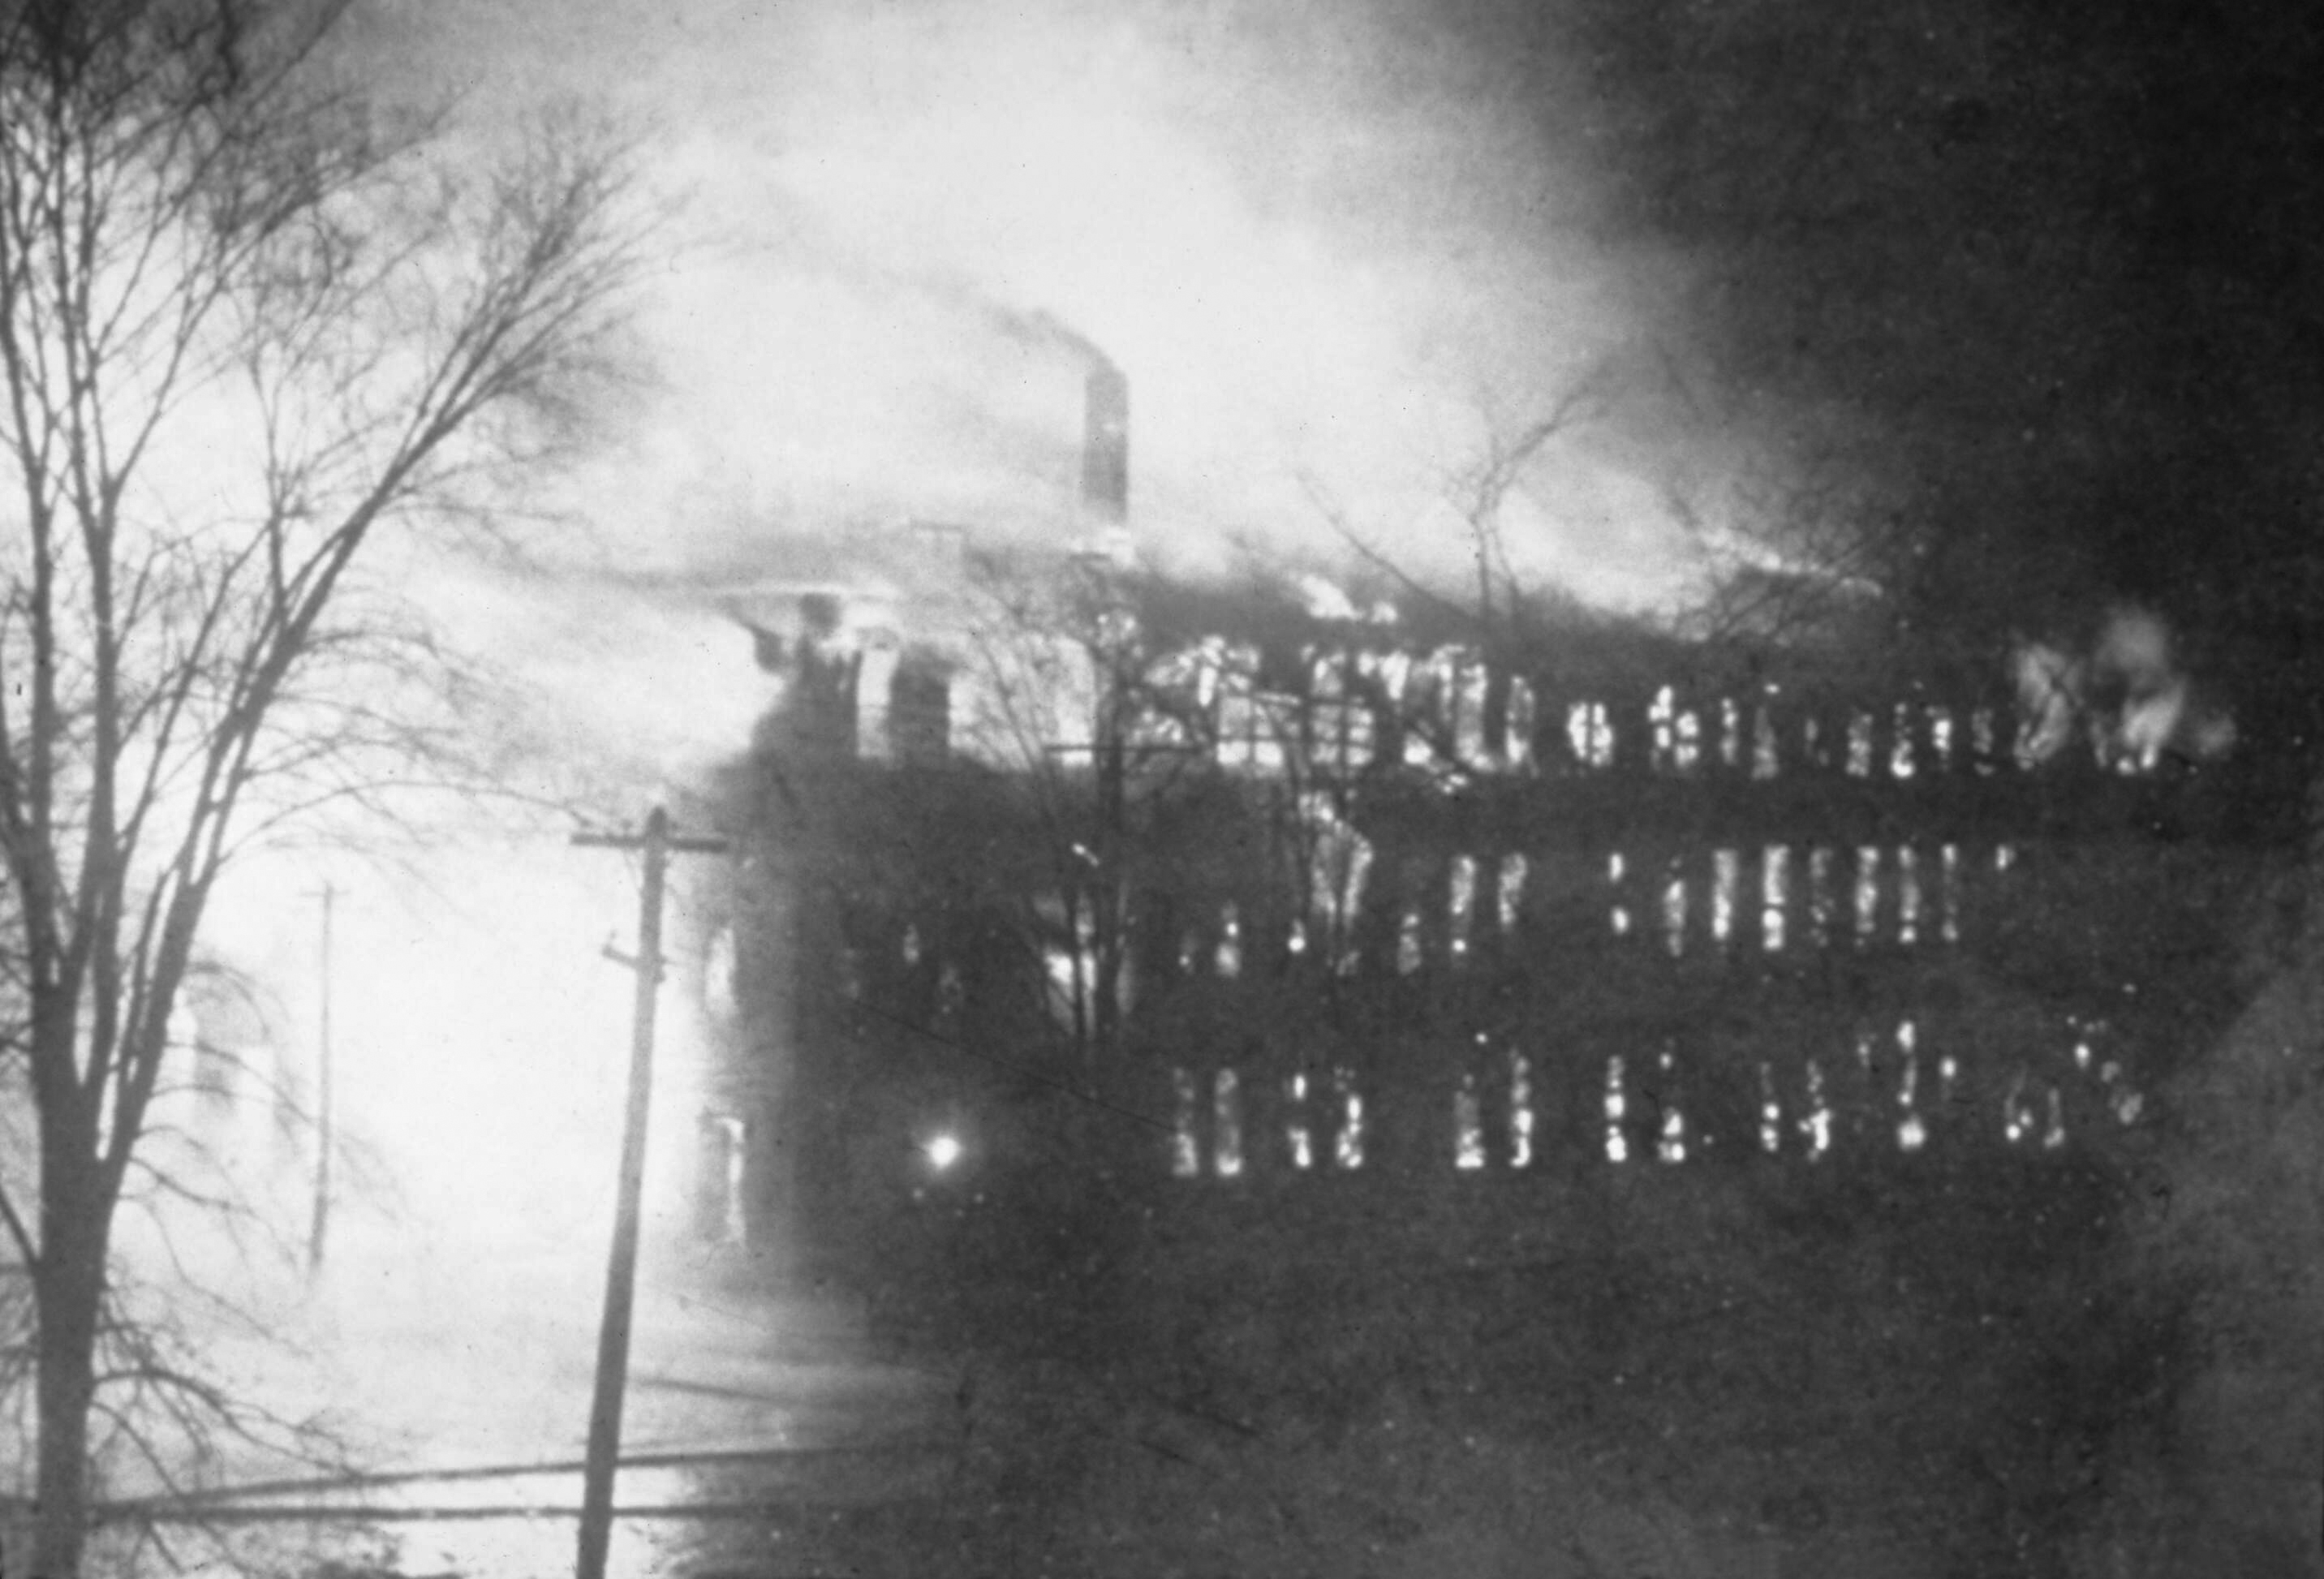
\includegraphics[width=1\linewidth]{images/review-and-herlad.jpg}
    \caption*{Spalenie budynku wydawnictwa Review and Herald, 30 grudnia 1902 r.}
    \label{fig:review-and-herald}
\end{figure}

\egw{Mam coś do powiedzenia naszym nauczycielom w odniesieniu do \textbf{nowej książki «The Living Temple»}. \textbf{Bądźcie ostrożni w popieraniu \underline{poglądów tej książki dotyczących osobowości Boga}}. Zgodnie z tym, jak Pan przedstawia mi te sprawy, \textbf{te poglądy nie mają poparcia Boga}. \textbf{Są one sidłem, które wróg przygotował na te ostatnie dni}. Myślałam, że zostanie to na pewno dostrzeżone i że nie będzie konieczne, abym cokolwiek o tym mówiła. \textbf{Ale ponieważ pojawia się twierdzenie, że nauki tej książki można poprzeć wypowiedziami z moich pism, jestem zmuszona zaprzeczyć temu twierdzeniu}. Mogą być w tej książce wyrażenia i poglądy, które są w zgodzie z moimi pismami. I mogą być w moich pismach liczne stwierdzenia, które wyrwane z kontekstu i interpretowane zgodnie z zamysłem autora «The Living Temple» wydawałyby się być zgodne z naukami tej książki. \textbf{Może to dawać pozorne poparcie twierdzeniu, że poglądy w «The Living Temple» są w zgodzie z moimi pismami}. \textbf{Ale broń Boże, żeby ta opinia przeważyła}}[Lt211-1903.1; 1903][https://egwwritings.org/?ref=en\_Lt211-1903.1]

Wielokrotnie siostra White stwierdzała, że prawdziwym problemem książki były poglądy \egwinline{\textbf{dotyczące osobowości Boga}}. Te poglądy nie są poparte stwierdzeniami z pism Ellen White i te właśnie poglądy \egwinline{\textbf{są pułapką, którą wróg przygotował na te ostatnie dni}}.

Bóg, ponownie w swojej opatrzności, rozwiązał ten konflikt. Kellogg przyjął naganę od posłanniczki Pana i przed zakończeniem rady oświadczył, że \textit{The Living Temple} zostanie wycofana z rynku\footnote{\href{https://forgottenpillar.com/wp-content/uploads/2022/04/Letter-A-G-Daniells-to-W-C-White-October-29-1903.pdf}{List: A. G. Daniells do W. C. White'a, 23 października 1903, str. 5}}. Jednak po konferencji rozmawiał prywatnie z przewodniczącym generalnej konferencji, bratem Arthurem G. Daniellsem, o swoich planach dotyczących książki. Poniżej przedstawiamy wybrane listy, ujawniające plany Kellogga dotyczące korekty \textit{The Living Temple}.

Ellen White nie była obecna na dorocznej konferencji w Waszyngtonie, ale jej syn, William C. White, w niej uczestniczył. Gdy konferencja się zakończyła, brat Arthur G. Daniells napisał poufny list do Williama C. White'a dotyczący planu dr Kellogga odnośnie do korekty jego książki:

\othersnodot{29 października 1903}

\othersnogap{Odkąd \textbf{rada została zamknięta}, czułem, że muszę napisać do Ciebie \textbf{poufnie w sprawie planów dr. Kellogga dotyczących korekty i publikacji «The Living Temple»} [...] On \normaltext{[Kellogg]} powiedział, że kilka dni przed przybyciem na radę, przemyślał tę sprawę i zaczął dostrzegać, że \textbf{popełnił niewielki błąd w wyrażaniu swoich poglądów}. Powiedział, że przez całą drogę był zatroskany o to, jak określić charakter Boga i jego związek z dziełami stworzenia...}

\begin{figure}[hp]
    \centering
    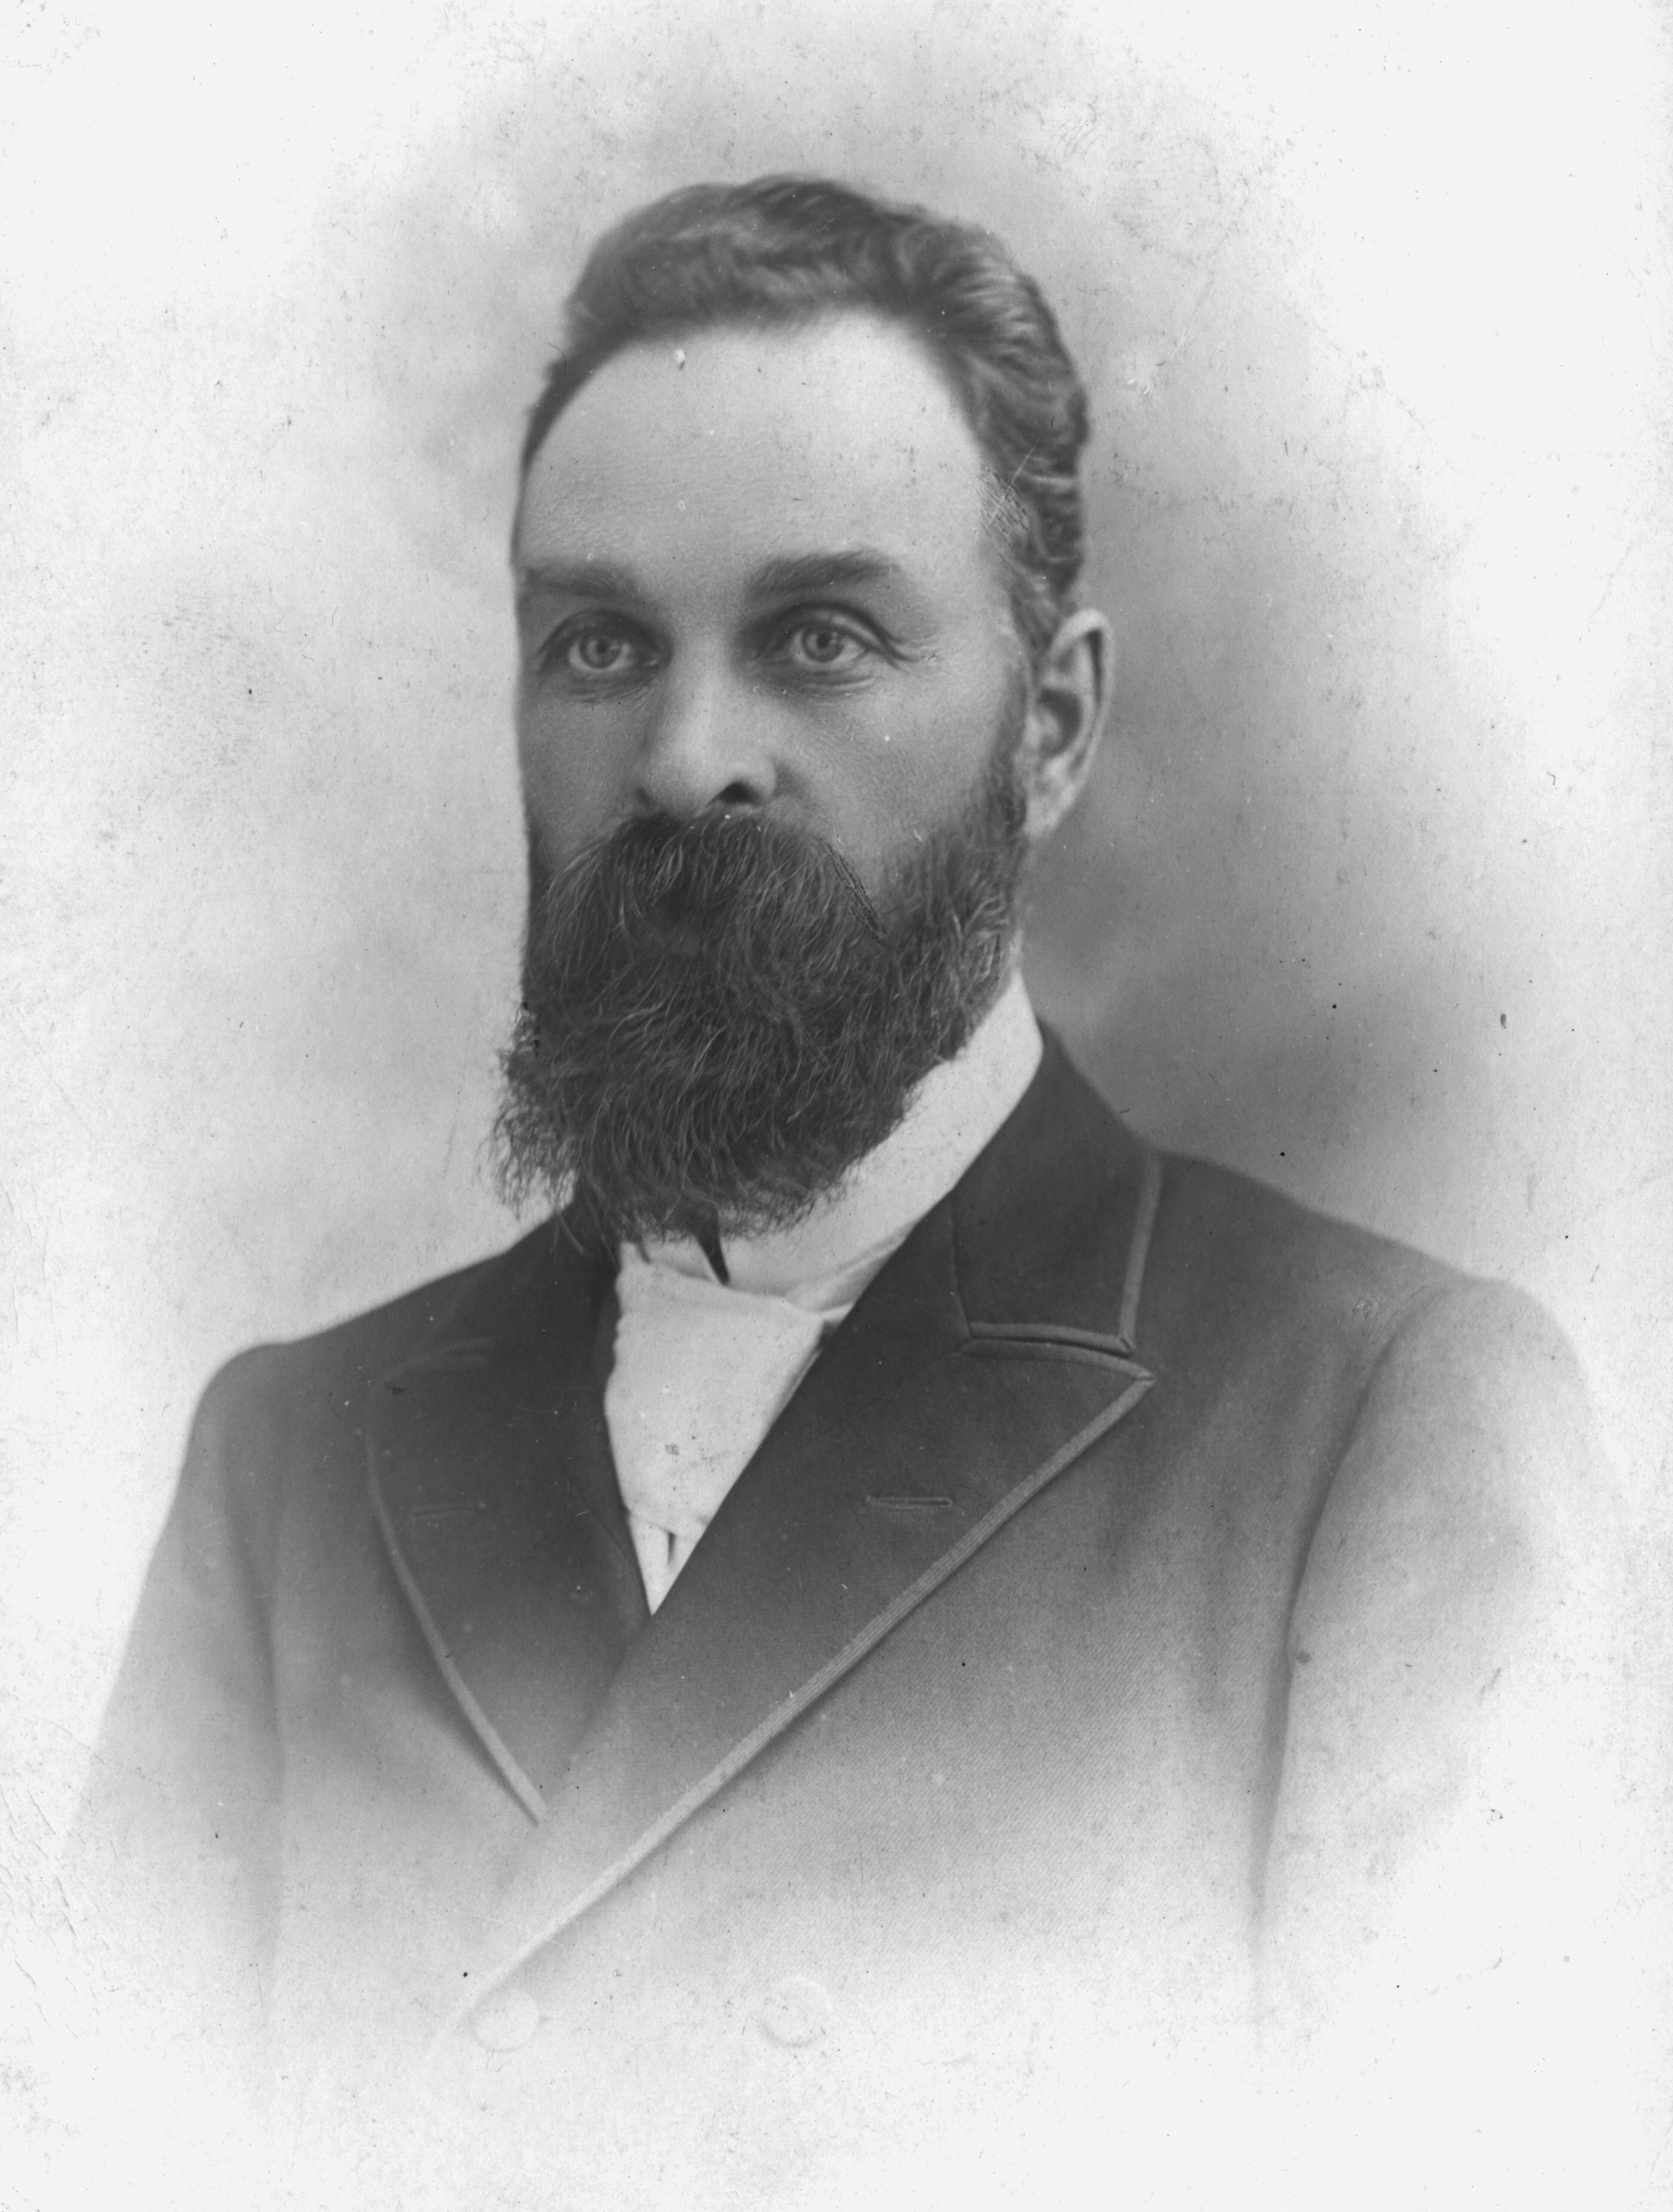
\includegraphics[width=1\linewidth]{images/daniels.jpg}
    \caption*{Arthur Grosvenor Daniells (1858-1935)}
    \label{fig:daniells}
\end{figure}

\othersnogap{\textbf{Następnie stwierdził, że jego wcześniejsze poglądy \underline{dotyczące trójcy} stanęły mu na drodze w złożeniu jasnego i całkowicie poprawnego oświadczenia; ale że niedługo potem \underline{zaczął wierzyć w trójcę} i mógł teraz całkiem wyraźnie zobaczyć, gdzie tkwił cały problem, i wierzył, że może wyjaśnić sprawę w satysfakcjonujący sposób}}

\othersnogap{\textbf{Powiedział mi, że teraz wierzy w \underline{Boga Ojca, Boga Syna i Boga Ducha Świętego}; a jego pogląd był taki, że to Bóg Duch Święty, a nie Bóg Ojciec, wypełnia całą przestrzeń i każdą żywą istotę. Powiedział, że gdyby  wierzył \underline{w to} przed napisaniem książki, to wyraziłby swoje poglądy bez wywoływania mylnego wrażenia, jakie teraz wywiera owa książka}}

\othersnogap{\textbf{Przedstawiłem mu zastrzeżenia, jakie znalazłem w tej nauce, i próbowałem mu pokazać, że nauka ta jest tak całkowicie sprzeczna z ewangelią, iż nie byłem w stanie sobie wyobrazić, jak można by ją poprawić, zmieniając tylko kilka wyrażeń}}

\othersnogap{Dyskutowaliśmy na ten temat dość długo w przyjaznej atmosferze; lecz byłem przekonany, że gdy się rozstaliśmy, doktor nie rozumiał ani siebie, ani charakteru swojego nauczania. Nie mogłem też pojąć, jak mógłby nagle zmienić zdanie i \textbf{w ciągu kilku dni \underline{poprawić książkę} tak, aby wszystko było w porządku}}[Letter: A. G. Daniells to W. C. White. October 29, 1903. pp. 1, 2][https://forgotten-pillar.s3.us-east-2.amazonaws.com/Letter-A-G-Daniells-to-W-C-White-October-29-1903.pdf]

Kellogg nie dostrzegał błędu w swoich poglądach, ale raczej w sposobie ich wyrażenia. Nie uważał, że jego poglądy były fałszywe, ale że sposób ich wyrażenia sprawił, iż książka dawała błędne wrażenie. Jednak najwyraźniej nie była to prawda. Jak stwierdziła siostra White, Kellogg miał problem z poglądami dotyczącymi \emcap{osobowości Boga} i tego, gdzie jest Jego obecność. Dlatego Kellogg zasugerował, że aby „\textit{poprawić książkę}”, doda trynitarne wyrażenia, ponieważ zaczął wierzyć w doktrynę o \textit{Trójcy}. W tym czasie Kościół Adwentystów Dnia Siódmego nie był trynitarny — doktryna o Trójcy nie była częścią \emcap{Fundamentalnych Zasad}, jak widzieliśmy wcześniej. Nie dziwi więc, że brat Daniells sprzeciwił się trynitarnej nauce i ją odrzucił, twierdząc, iż była ona \othersnodot{tak całkowicie sprzeczna z ewangelią}. Poprawienie książki poprzez zmianę kilku wyrażeń nie rozwiązałoby głównego jej problemu: poglądów na temat \emcap{osobowości Boga}.

W opisanych wydarzeniach i w odpowiedzi Williama White'a do brata Daniellsa możemy zobaczyć, dlaczego siostra White napisała \textit{Special Testimonies}. William White odpowiedział bratu Daniellsowi 4 listopada 1903 roku:

\othersnodot{Drogi Bracie,}

\othersnogap{\textbf{\underline{Matka i ja} właśnie przeczytaliśmy Twój list z \underline{29 października}, w którym mówisz o \underline{różnych planach zaproponowanych celem korekty i ponownego wydania «The Living Temple»}}}

\othersnogap{Byliśmy mile zaskoczeni wiadomością, że dr. Kellogg wycofa tę książkę z rynku, \textbf{i jest nam niezmiernie przykro, że jego myśli powracają do planu jej korekty, \underline{Matka wyraziła się dość stanowczo w tej sprawie; uważa to za bezowocne przedsięwzięcie}}. Myślę, że wkrótce napisze do Ciebie, wyrażając swoje poglądy na ten temat}

\othersnogap{\textbf{... Uważam, że będzie konieczne \underline{wydanie wkrótce specjalnego Świadectwa}, które musi zawierać pełne i jasne stanowisko w pozytywnym aspekcie tej kwestii, jak również artykuły wskazujące na błędy w nauczaniu tych, którzy odeszli od prawdy poprzez czarujące i zwodnicze teorie}}[\href{https://ellenwhite.org/letterbooks/555}{List od W.C. White'a do A.G. Daniellsa, 4 listopada 1903,} (str. 458)]

\begin{figure}[h]
    \centering
    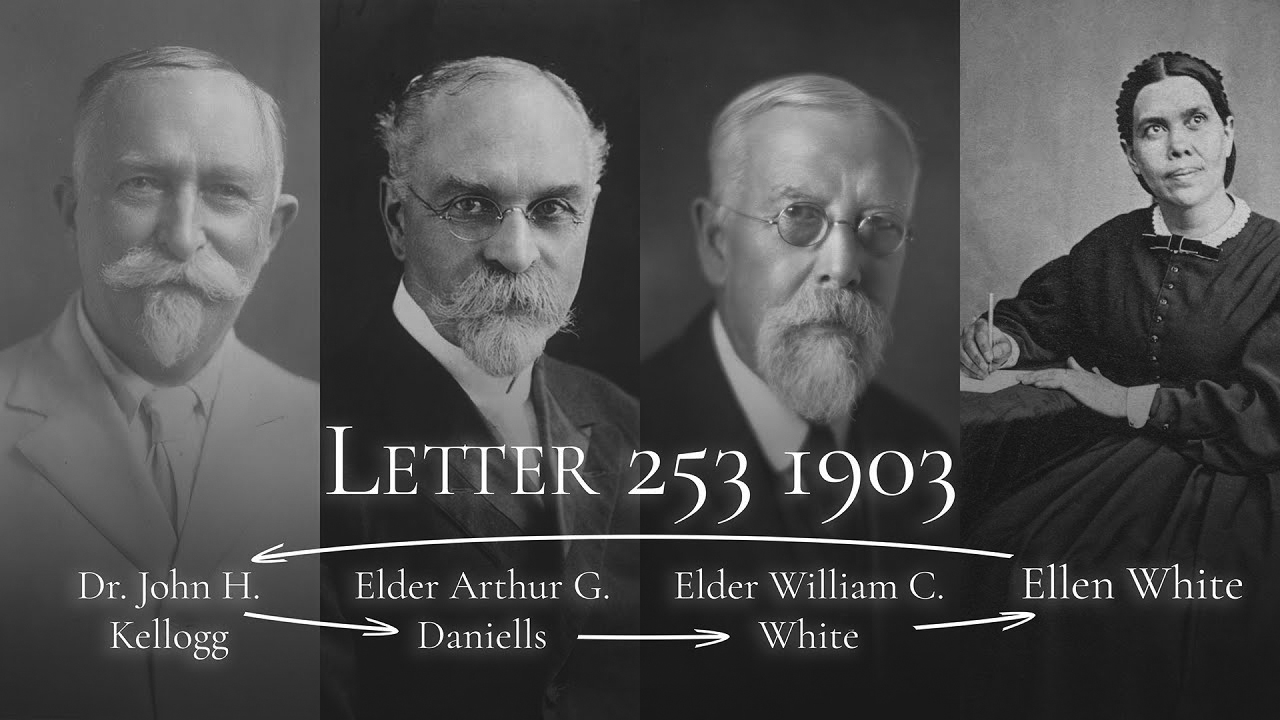
\includegraphics[width=1\linewidth]{images/correspondance.jpg}
    \caption*{Łańcuch korespondencji pomiędzy A. G. Daniellsem, W. C. White'em, Ellen White i dr. Johnem H. Kelloggiem.}
    \label{fig:corespondance}
\end{figure}

Oto dowód, że siostra White była zaznajomiona z zamiarami dr. Kellogga dotyczącymi korekty \textit{The Living Temple} oraz jego wiarą w doktrynę o Trójcy. Według słów Williama wypowiedziała się bardzo stanowczo w tej sprawie. Uznała to za bezowocne przedsięwzięcie. Z tego powodu konieczne było wydanie wkrótce specjalnego Świadectwa. I tak się stało. W ten sposób w 1904 roku opublikowano \textit{Testimonies for the Church Containing Letters to Physicians and Ministers Instruction to Seventh-Day Adventists}, zawierające listy do lekarzy i kaznodziejów związanych z kryzysem Kellogga.

Mówiąc: \othersnodot{\textbf{\underline{Matka i ja} właśnie przeczytaliśmy Twój list z \underline{29 października}}}, William zaświadczył, że siostra White była w pełni świadoma zamiarów Kellogga i jego trynitarnych przekonań. Po przeczytaniu listu Daniellsa napisała bezpośrednią odpowiedź do dr. Kellogga. Ten list to \textit{Lt253-1903}. Jest to bardzo znaczący i odkrywczy list, ponieważ jasno pokazuje, jak prorokini odnosiła się do doktryny o Trójcy. Podkreśliła doktrynę o \emcap{osobowości Boga} zawartą w \emcap{Fundamentalnych Zasadach}. Istnieją uderzające podobieństwa między tym listem a dziesiątym rozdziałem \textit{Special Testimonies}, „Fundament naszej wiary”.

\begin{titledpoem}
    \stanza{
        W „Świątyni” Kelloga sidło leżało, \\
        Przedstawienie Boga White nie pasowało. \\
        Jego słowa na temat osobowości Boga \\
        Były sofizmatami wręcz prosto od wroga.
    }

    \stanza{
        Nie będą naprawione żadne błędy stare \\
        Przez lekką korektę czy też w Trójcę wiarę. \\
        Gdyż osobowość Boga wyraźna i czysta — \\
        W tę prawdę winien wierzyć każdy adwentysta.
    }

    \stanza{
        Pomimo zastawionych sideł przeciwnika \\
        Niech prawda o Bogu z oczu nam nie znika. \\
        Fundament nasz musi bezpieczny pozostać \\
        I wsparty przez Biblię na wieki się ostać.
    }
\end{titledpoem}

